
\label{chap:experimental_results}


%FIXME: add text here

\section{Memory Synchronizer}

    This section describes the various tests performed on the full/empty memory synchronizer used within the PDP firmware to synchronize data transitioning across clock domains. First, it discusses simulation results obtained through a full behavioral simulation of PDP. Secondly, it discusses using the memory synchronizer in a test setup and pitfalls that occurred with earlier implementations.

    \subsection{Simulation}
        Figure~\ref{fig:full_empty_sim} shows the simulated results of the full/empty memory synchronizer when transitioning to full and back to empty per clock cycle for a writer and reader operating at \mbox{35.75 Mhz} and \mbox{200 Mhz}, respectively. For discussion about each signal and the expected internal behavior see Chapter~\ref{sec:memorysync}. Each state transition in the simulation should look similar to the state transitions shown in Table~\ref{tbl:full_empty_circuit_states}.

        \begin{figure}[t]
            \centering
            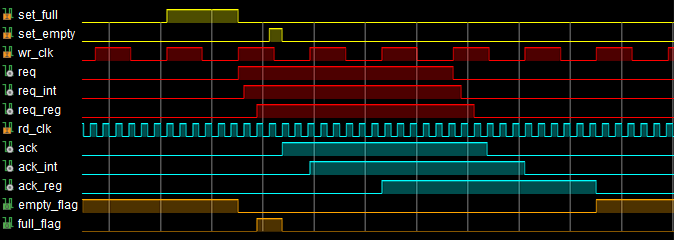
\includegraphics[width=1.0\textwidth]{fig/full_empty_sim.png}
            \caption{Full/Empty Circuit Simulation}
            \label{fig:full_empty_sim}
        \end{figure}

        The circuit holds a steady state until the {\it set full} signal is toggled for a single {\it write clock} cycle. On the next {\it write clock} cycle, the {\it req signal} transitions high and the {\it empty flag} transitions low. Then the data is moved to the {\it read clock} domain using the two flip-flop synchronizer scheme discussed in the implementation details. At the next rising edge of the {\it read clock}, the data is latched into {\it req internal} which is an internal metastable register. Due to the speed difference between write and read clock speed, the data latches into the register quickly. Following this, a cycle later, the data is clocked into {\it req reg} which completes the {\it read clock} domain transition causes the {\it full flag} to transition high.

        Once any corresponding buffer data is handled by the PDP firmware, the {\it set empty} signal is toggled for a single {\it read clock} cycle. This causes the {\it ack} signal to transition high. Then the data is moved to the {\it write clock} domain using the two flip-flop synchronizer scheme discussed in the implementation details. At the next rising edge of the {\it write clock}, the data is latched into {\it ack internal}. Following this, a cycle later, the data is clocked into {\it ack reg} which completes the {\it write clock} domain transition. Notice that it takes much longer to transition data from the {\it read clock} domain to the {\it write clock} domain than vice versa. This is due to the slow write clock.

        A {\it write clock} cycle later, {\it req} transitions low. Subsequently, it transitions to the {\it read clock} domain just as before. Following this, the {\it ack} line is lowered and transitions to the {\it write clock} domain just as before. At the same time, the {\it empty flag} transitions high, and the circuit is in the state it began in.

        This follows the expected state transitions from Table~\ref{tbl:full_empty_circuit_states} with the only notable distinction being that transitions across clock domains take different amounts of time depending on the destination.

        In practice, a complete double handshake takes many cycles to complete which could lead to undesired overflow behavior. In PDP, overflow issues are mitigated by allocating enough internal buffers to allow for there to always be a buffer available for a writer to fill.

        Additionally, the use of the two flip-flop synchronizer means that it takes more than a single {\it read clock} cycle for the {\it full flag} to raise; however, given that the pixels of an IRLED array take many {\it read clock} cycles to charge, this does not pose a problem. Moreover, in practice, the {\it full flag} will transition in between two to three cycles of the reader clock depending on where the rising edge of the reader clock falls relative to the transitioning of the {\it req} signal.

        Figure~\ref{fig:full_empty_row_sim} shows the simulated results of the full/empty memory synchronizer for multiple pixels. The large gaps of time between transitions to full are due to there being multiple buffers available as discussed above. This indicates that at the simulated rates no overflow can occur. In practice, it would be possible for overflow to occur if the write clock speed was close to the read clock speed; however, due to the maximum possible write speed for HDMI only being \mbox{148.5 MHz} and the hiding of clock domain crossinglatency via multiple buffers, a \mbox{200 Mhz} input clock is sufficient for correct behavior.

        \begin{figure}[t]
            \centering
            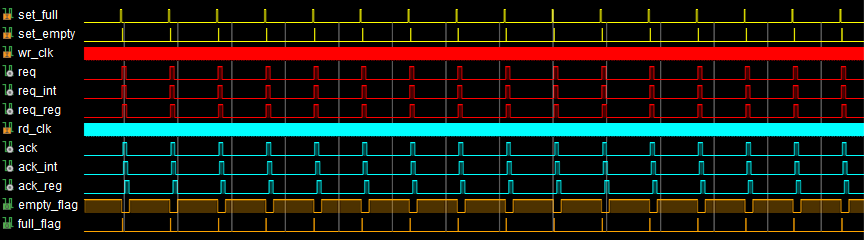
\includegraphics[width=1.0\textwidth]{fig/full_empty_row_sim.png}
            \caption{Full/Empty Circuit Multiple Pixel Simulation}
            \label{fig:full_empty_row_sim}
        \end{figure}

    \subsection{Verification}

%\begin{figure}
%    \centering
%    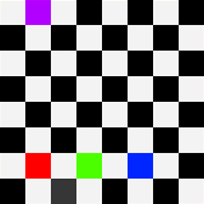
\includegraphics{fig/checker.png}
%    \caption{Checker Input Image}
%    \label{fig:checker_pattern}
%\end{figure}
%
%\begin{figure}
%    \centering
%    
\includegraphics{fig/random_noise.png}
%    \caption{Random Noise Input Image}
%    \label{fig:random_noise}
%\end{figure}

\section{Firmware}
    This section discusses behavioral simulation results from the PDP firmware implementation and experimental results obtained from running the firmware on actual IRLED arrays.

    \subsection{Simulation}
    This section provides captures of simulation inputs and outputs to show how packets arrive and are processed by the firmware architecture.

    In Figure~\ref{fig:input_example} simulated HDMI is shown. When video data enable (write enable) transitions high words of data representing PDP packets start to stream in. These are indicated by packet ID, X start, X end, Y start, Y end, and Packet Data. Each word would be stored in an SCB slot as indicated in the previous section. The final piece of data indicated is a reset packet. Note, that the data prior to Packet ID would be ignored as it does not represent a valid PDP command. It would be discarded by the valid controller.

    \begin{figure}
        \centering
        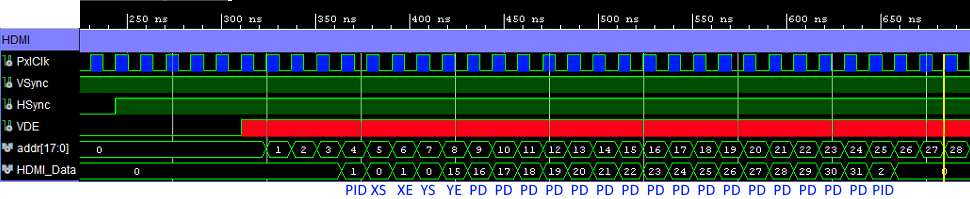
\includegraphics[width=1.0\textwidth]{fig/pdp_input_example.png}
        \caption{PDP Single HDMI Input Example Simulation}
        \label{fig:input_example}
    \end{figure}

    Figure~\ref{fig:output_example} shows the final output driven to the array. Highlighted in red is data from the write enable packet. Note, all values out are up shifted by 5 bits to be received by the DACs in the system. Additionally, the values are shown in reverse order from the input diagram. For example, 992 corresponds to the value of 31 on the input side. In purple the reset packet is shown with two stages of array writes. In the first stage, load line goes low. In the second stage the load line transitions high. The states shown are the transitioning of the state machines discussed in Chapter~\ref{sec:state_machines}.

    \begin{figure}
        \centering
        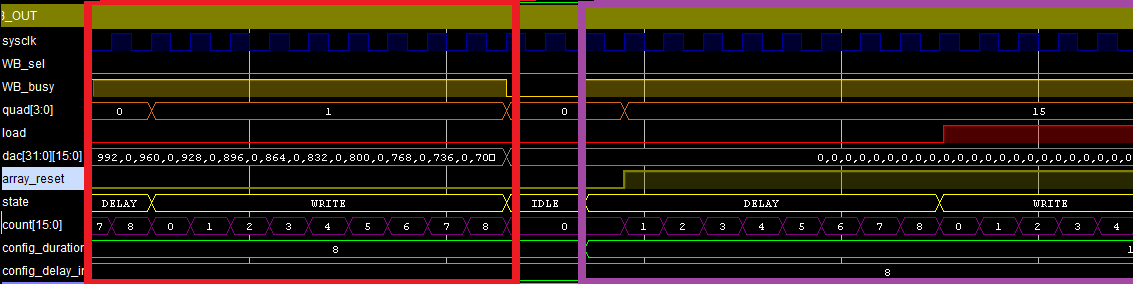
\includegraphics[width=1.0\textwidth]{fig/pdp_output_example.png}
        \caption{PDP Output Example Simulation}
        \label{fig:output_example}
    \end{figure}

    \subsection{Characterization}
        This section shows select results of running the PDP firmware on an NSLEDS array to characterize its behavior. Namely, whether it correctly draws to an array and whether it performs better than earlier firmware incarnations. Some non-uniformity correct imagery is also shown which indicates the PDP firmware is capable of drawing full imagery correctly. Though, only a few results are shown here, the PDP firmware has been run on multiple NSLEDS and HDILED arrays to collect data and characterize the arrays themselves. As of this writing, it has been used in daily operations with my research group's IRLED arrays for over a year and is the primary firmware in use today.

        \subsubsection {Array Maps}
            In order to characterize whether the behavior of PDP is consistent with older firmware (called SNAP) and has reproducible results between runs, a number of different array characterization tests were performed on an NSLEDS array. One test is to collect an array map which is performed by doing a sweep of array pixels by outputting light to each pixel separately over multiple frames and capturing the result. Typically, this is done using grids to speed up data collection. An example grid for a partial frame is shown in Figure~\ref{fig:grid_sweep}. Defective pixels on an array will have low light output or have inconsistent brightness from run to run. This could also happen if a firmware contained internal timing issues as well. Comparing a test firmware with a known good reference firmware can rule out firmware issues in the advent of this type of poor array behavior.

            \begin{figure}[t]
                \centering
                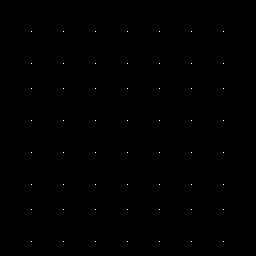
\includegraphics{fig/grid.jpg}
                \caption{Pixel Sweep Grid}
                \label{fig:grid_sweep}
            \end{figure}

            Figure~\ref{fig:array_map_pdp} shows an array map collected from the PDP firmware and Figure~\ref{fig:array_map_snap} shows an array map collected from the older SNAP firmware. In each figure, array data collected using an IR camera is shown on the left with a camera count scale on the right. Camera counts are an uncalibrated measure of IR intensity that can mapped to apparent temperature when calibrated. At a glance each image appears to be the same; however, there are slight differences in behavior between the firmwares in that PDP has a slightly higher light output. The dark regions of each map are simply dead pixels on the array and do not reflect the firmware. More than half of the particular array is non functioning. The repeating patterns of horizontal lines that can be seen are the result of slow DAC channels on an array. Every 32 columns there are 2 channels which take longer to settle and that can be seen in these results, as these channels have no fully settled. This is due to design flaw on early arrays which resulted in higher capacitance on those lines. Overall, the PDP results are as expected.

            \begin{figure}[t]
                \centering
                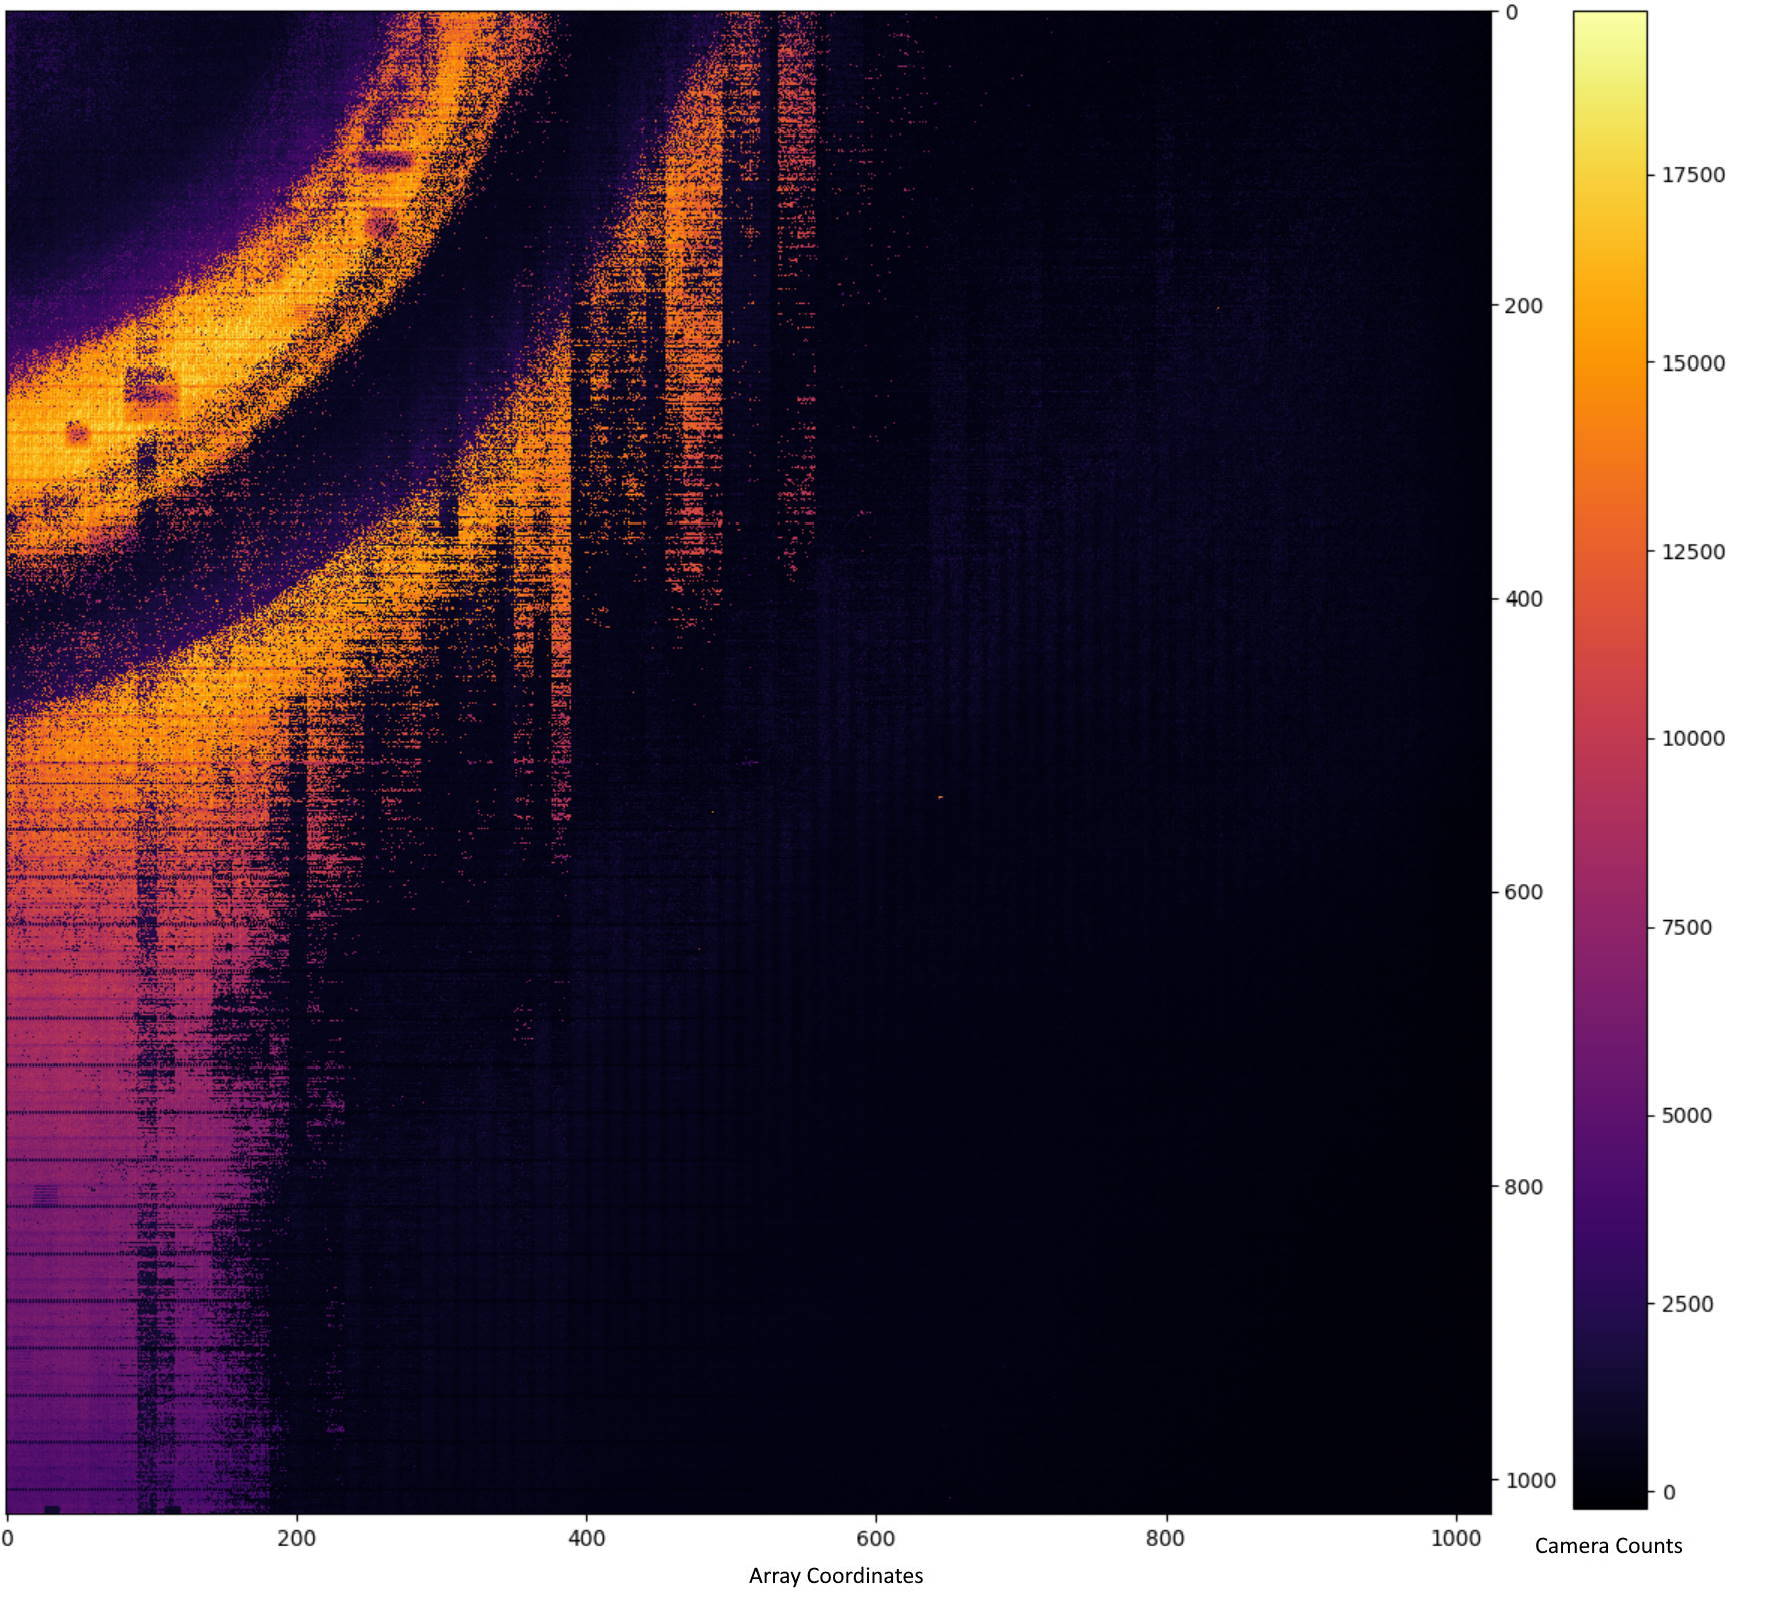
\includegraphics[width=1.0\textwidth]{fig/array_map_pdp.jpg}
                \caption{PDP Firmware Array Map}
                \label{fig:array_map_pdp}
            \end{figure}

            \begin{figure}[t]
                \centering
                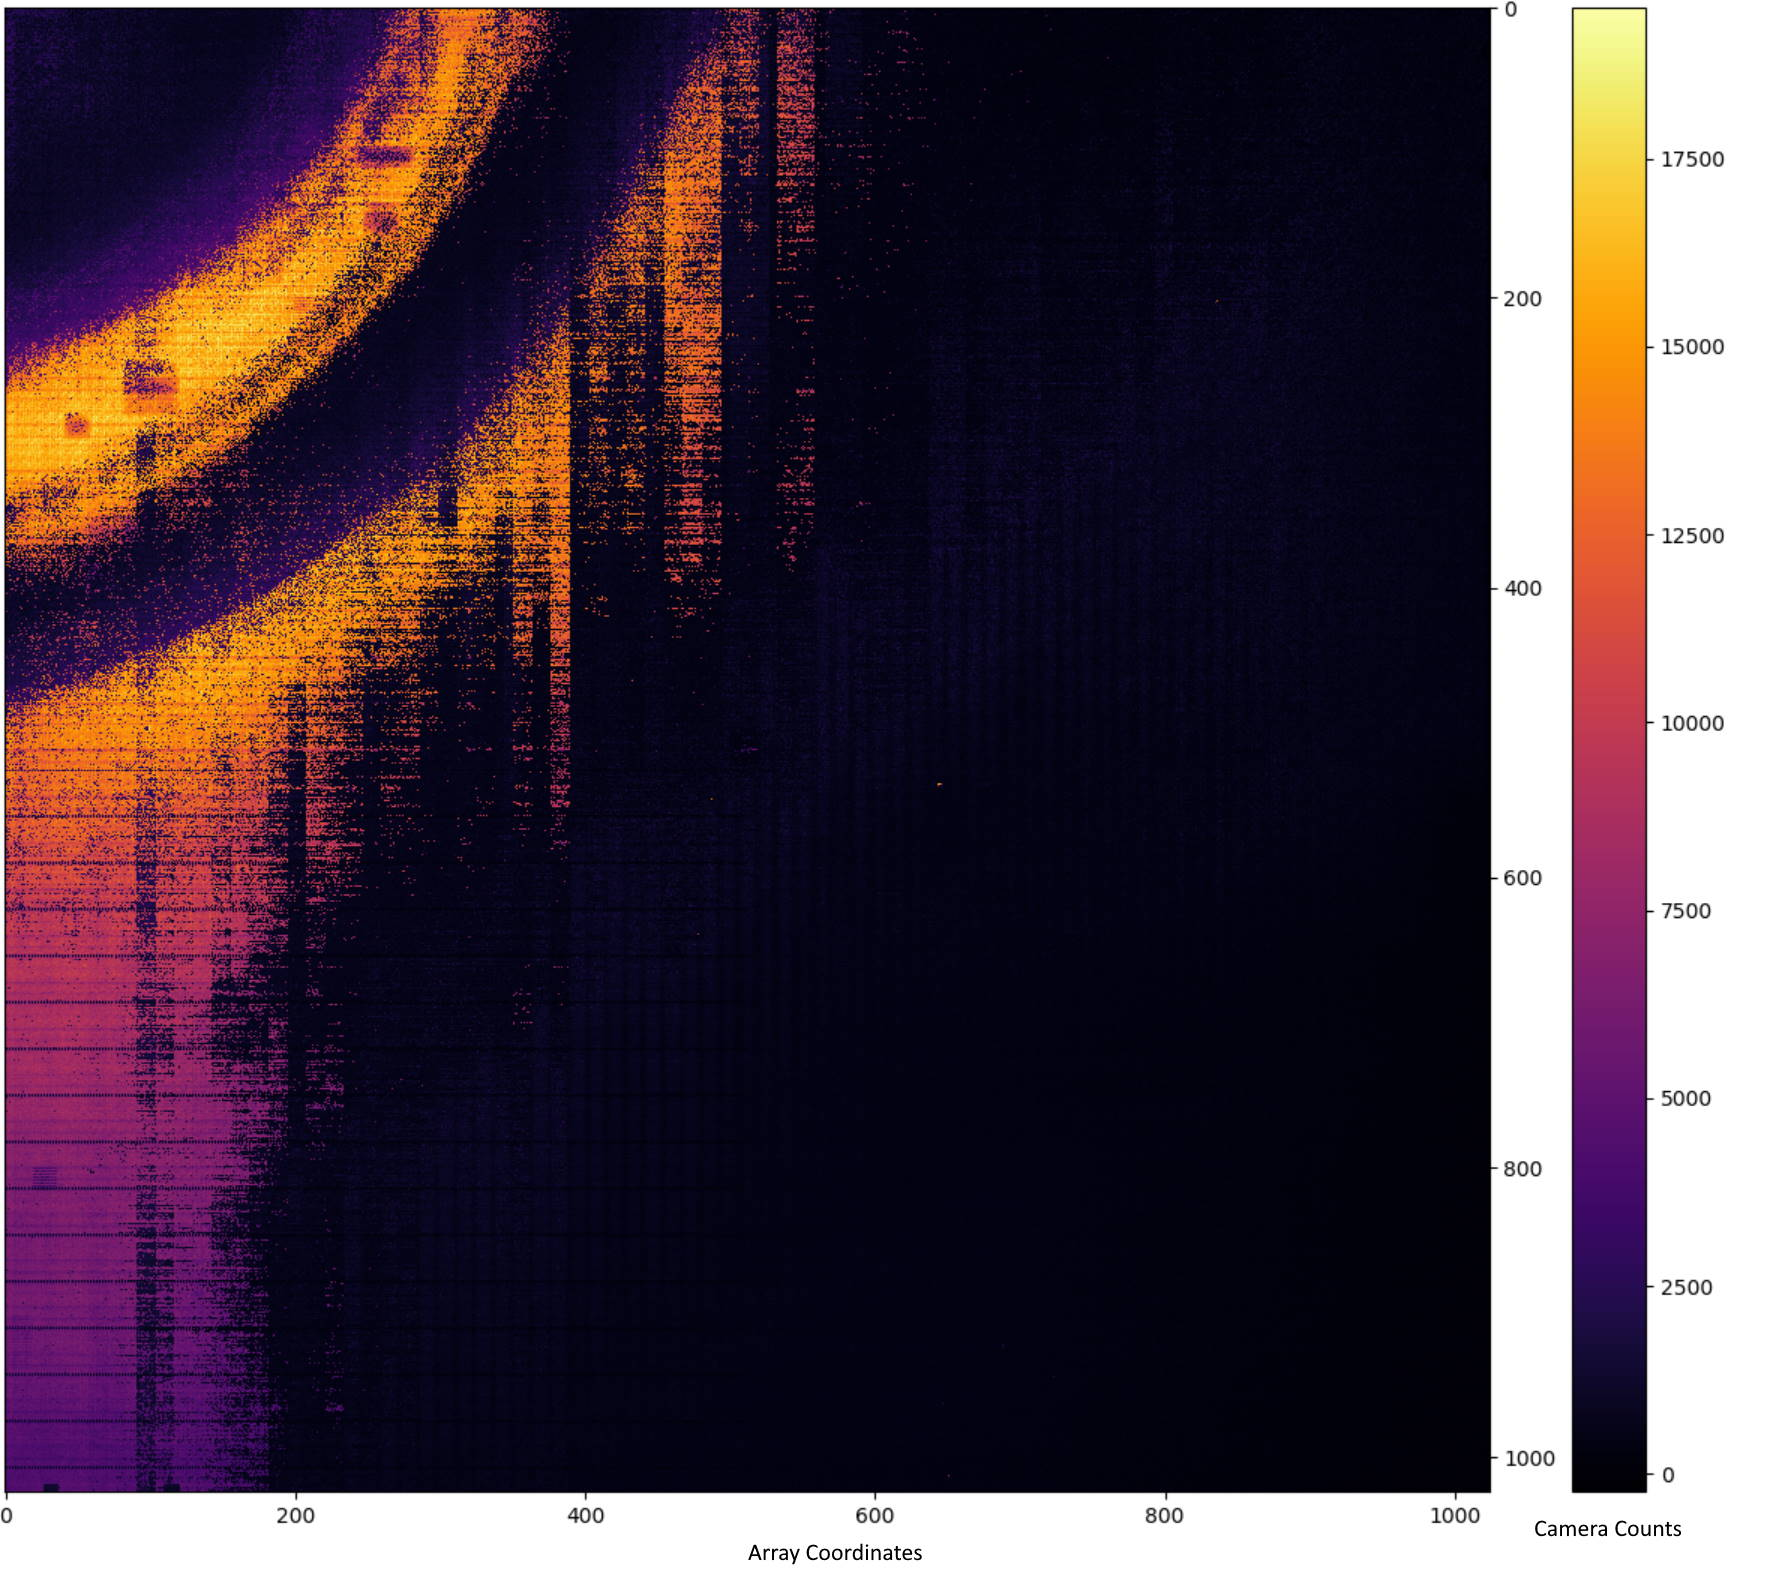
\includegraphics[width=1.0\textwidth]{fig/array_map_snap.jpg}
                \caption{SNAP Firmware Array Map}
                \label{fig:array_map_snap}
            \end{figure}

        \subsubsection{Fractional Difference Maps}

            Another test is to collect multiple array maps and take the fractional difference between them to see the percent difference in light output between runs. This allows for the consistency of light output to be characterized. A large difference could indicate problems with the pixels of an array, analog chain, or firmware behavior. Small differences indicate that the pixels of an array are more consistent between runs. Differences in behavior between firmwares (or firmware revisions) would be indicative of variances in signal timing. In this case, a larger variance would indicate less precise timing within the firmware. Some variance is expected is due to camera focus, noise, and physical vibration. The particular IR camera used to collect data in this setup utilizes a motorized reversed-stirling cryo-cooler. These are often utilized for cooling detectors within thermal imaging systems\cite{Organ1999}. These induce a physical vibration which can result in noise within collected camera imagery.

            Figure~\ref{fig:fractional_difference_pdp} shows a fractional difference map for the PDP firmware and Figure~\ref{fig:fractional_difference_snap} shows a fractional difference map for the older SNAP firmware. The dark blue areas indicating zero difference are simply dead regions of the array similar to the earlier results. The red areas of high variance are due to those pixels being located on marginal portions of the array specifically along non-functioning edges. In practice for displaying imagery, these areas would be marked as defected and not driven.

            \begin{figure}[t]
                \centering
                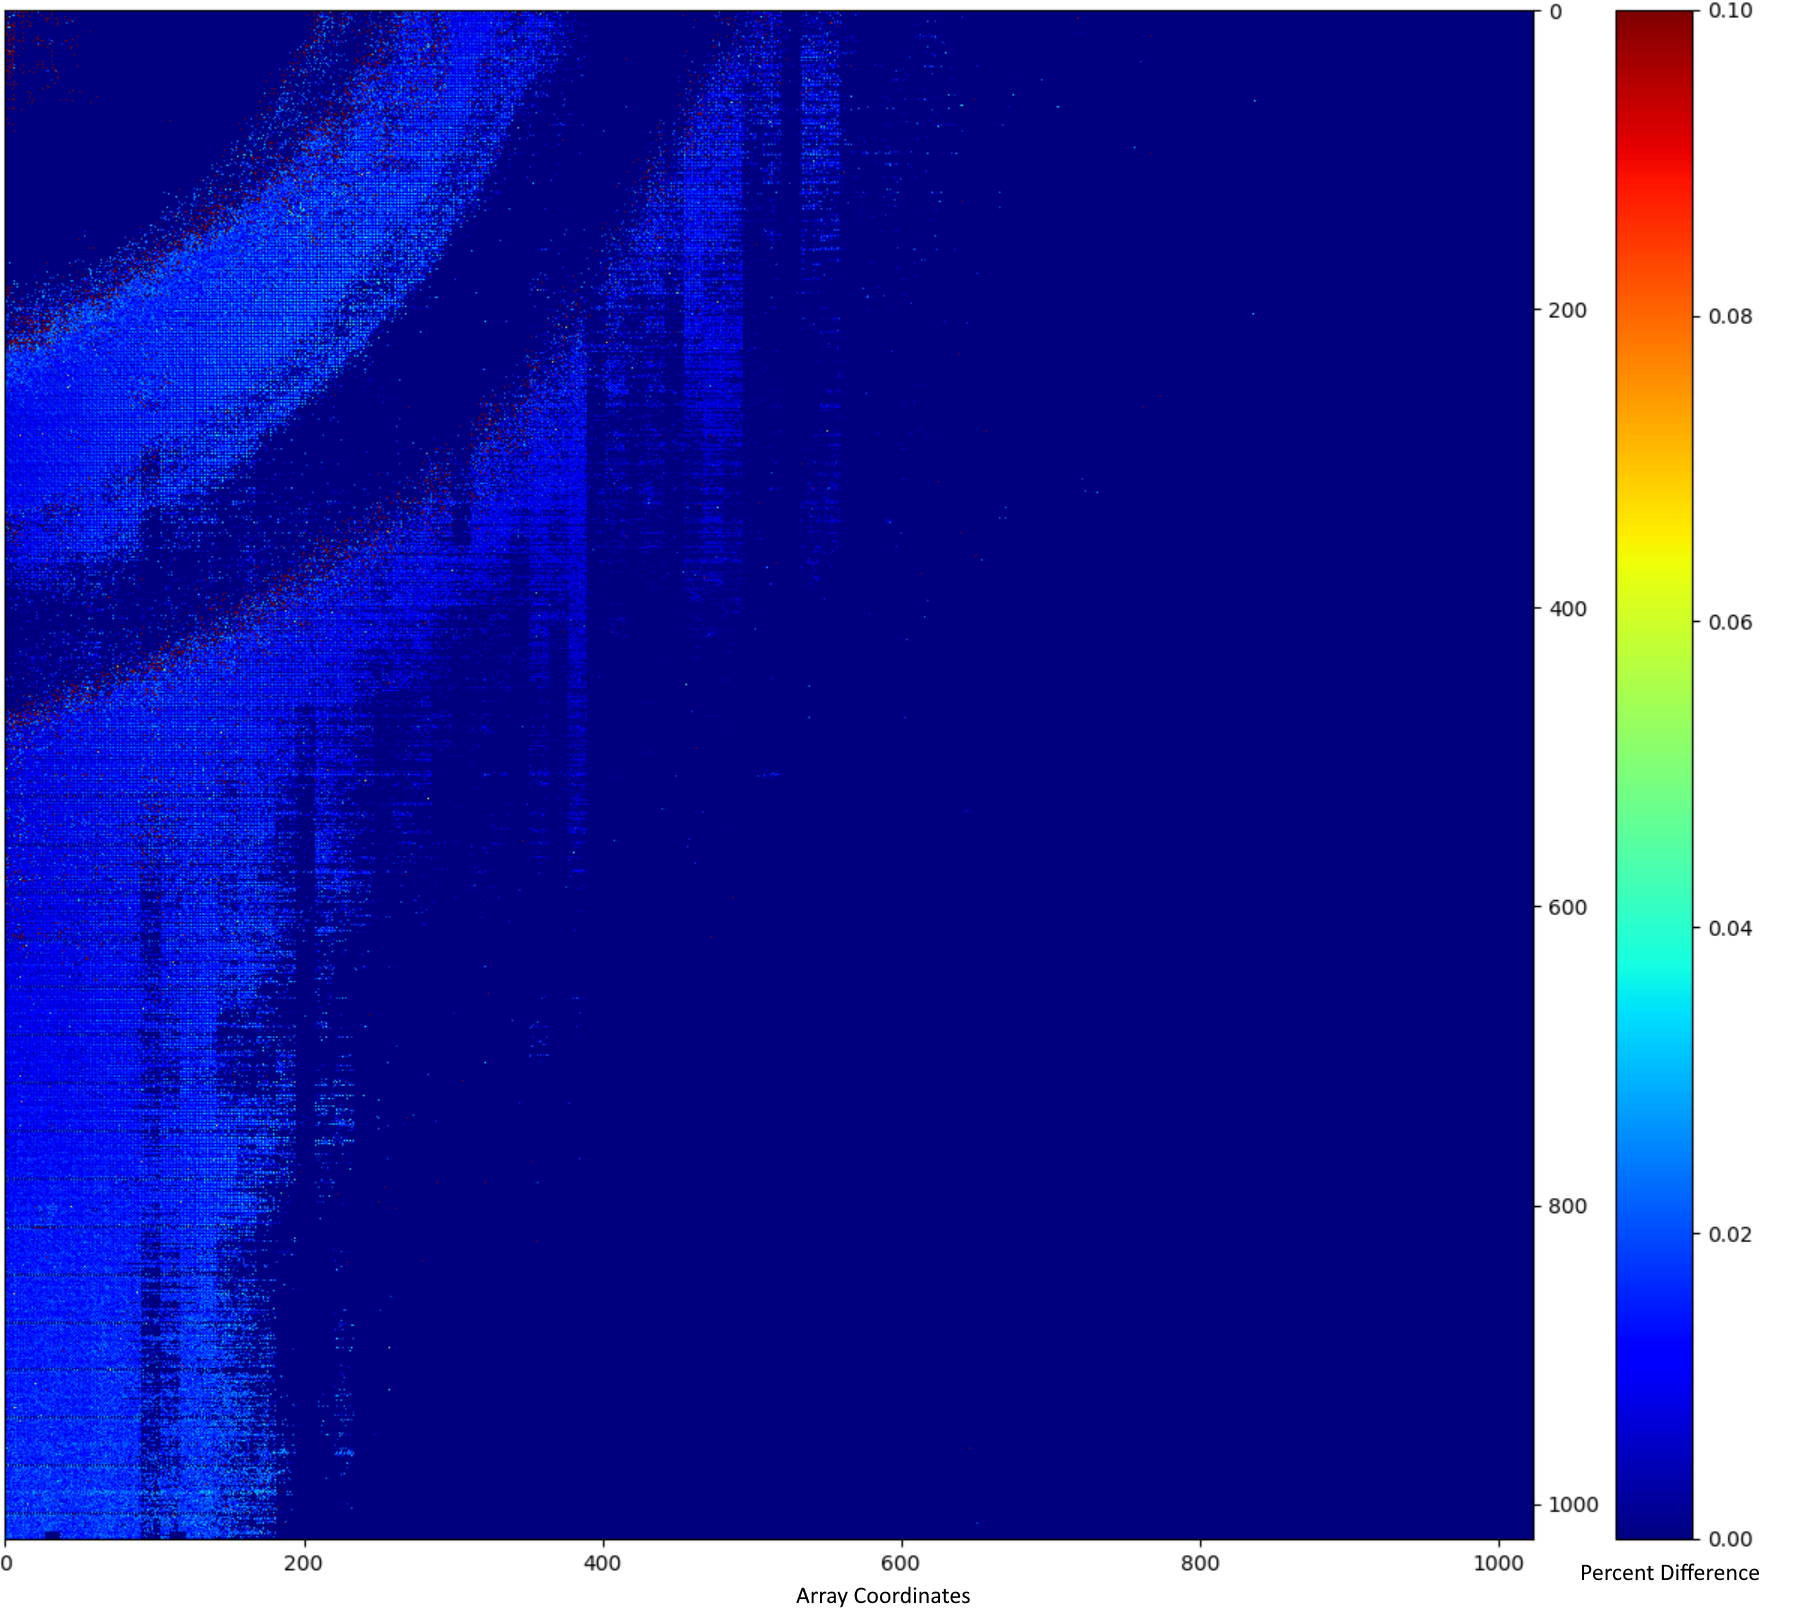
\includegraphics[width=1.0\textwidth]{fig/fractional_difference_pdp.jpg}
                \caption{PDP Firmware Fractional Difference Map}
                \label{fig:fractional_difference_pdp}
            \end{figure}

            \begin{figure}[t]
                \centering
                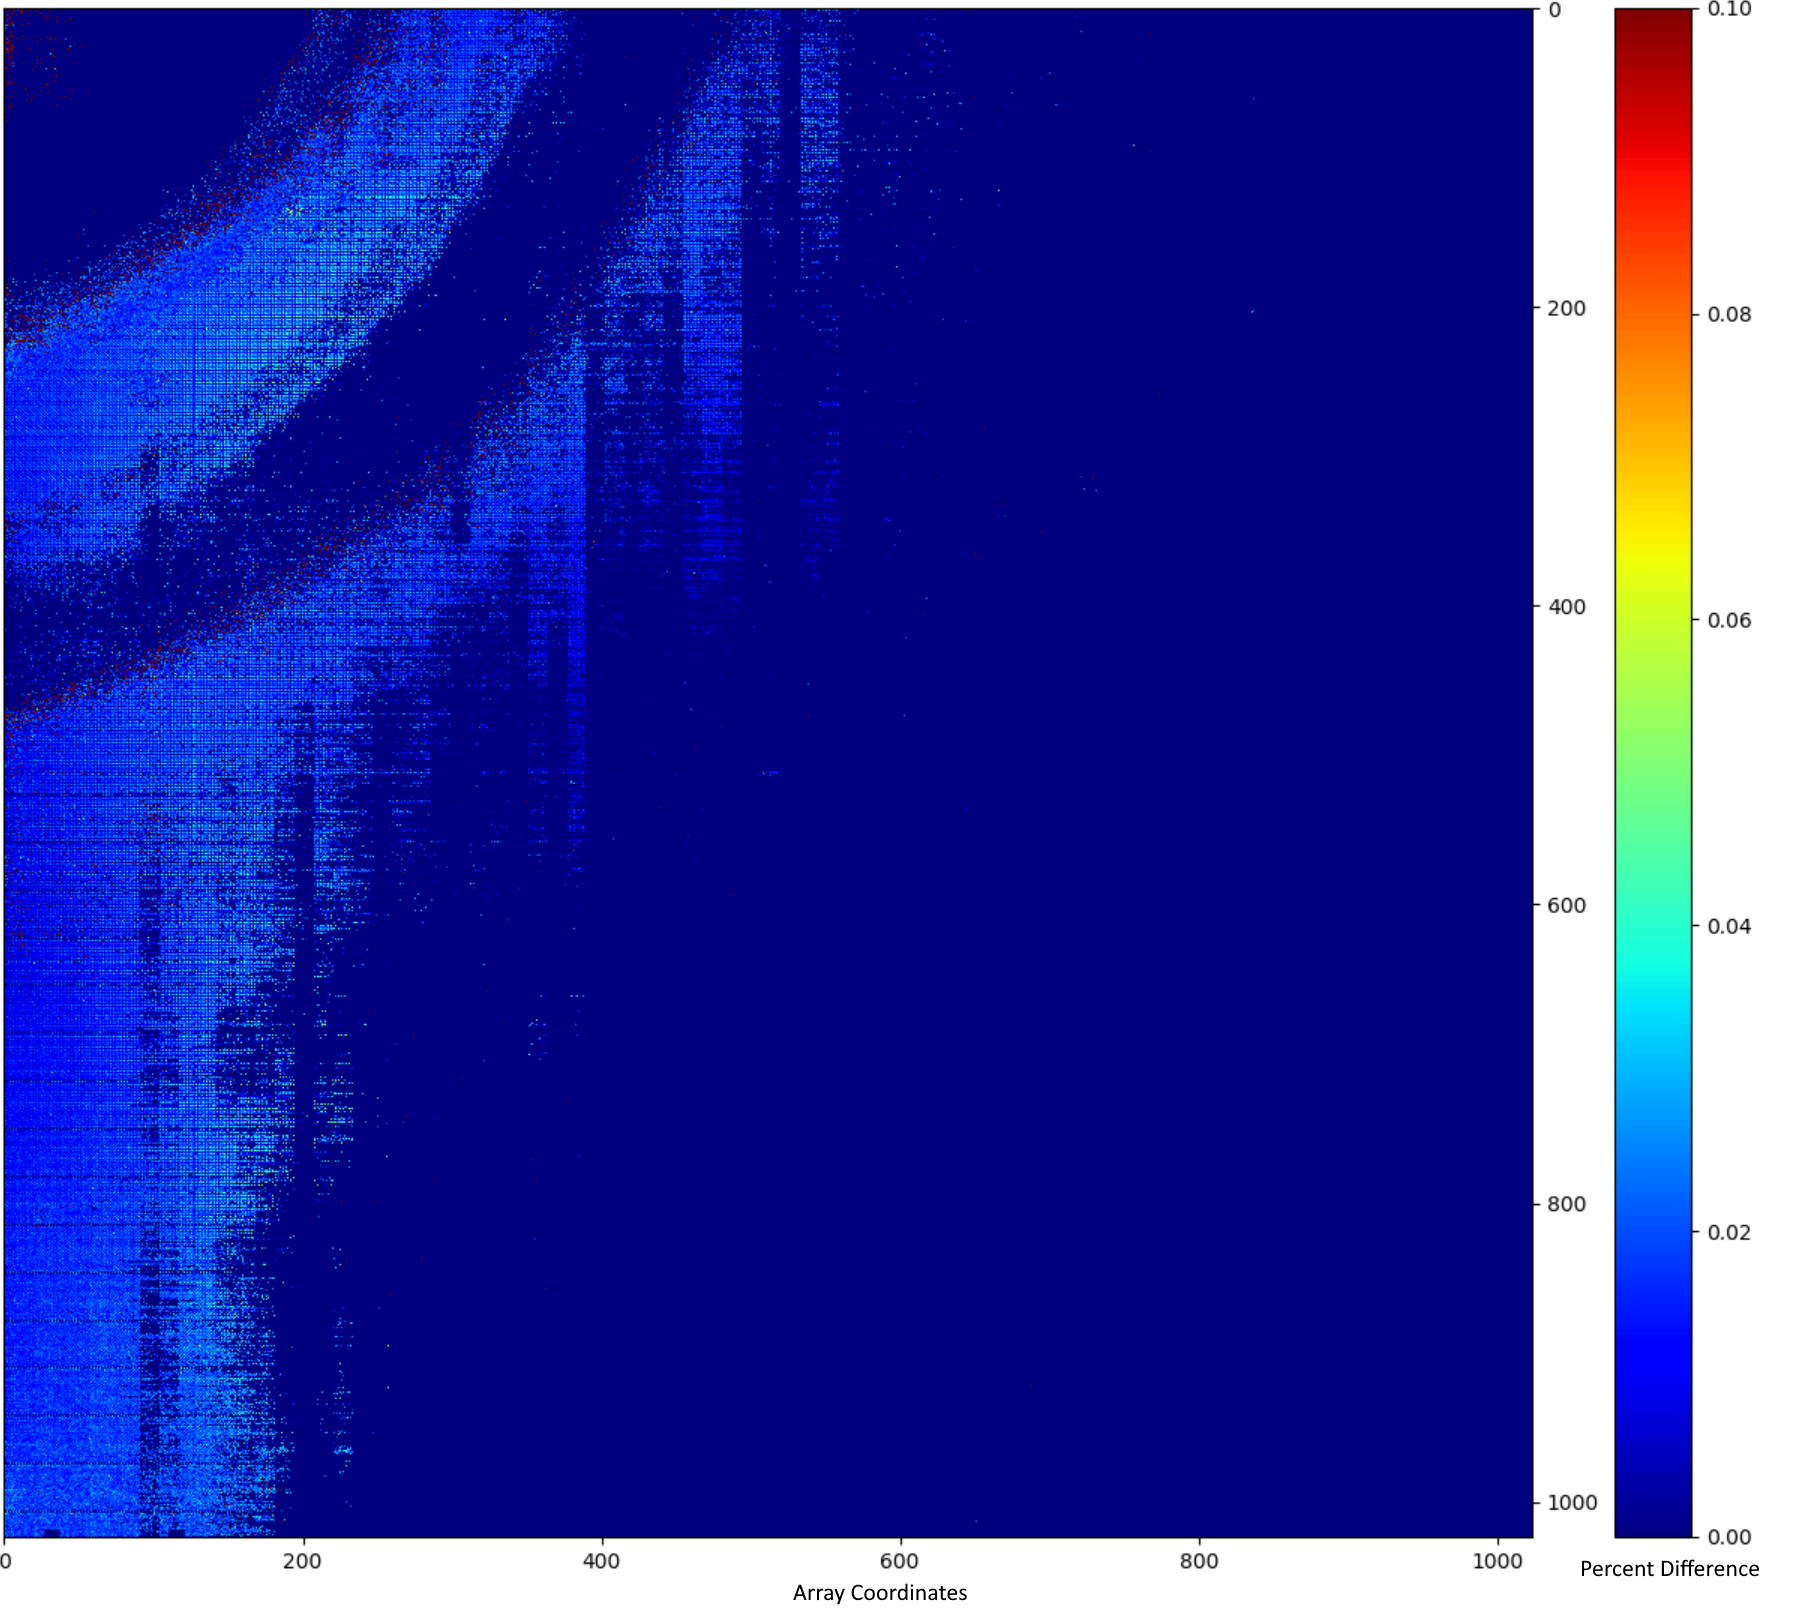
\includegraphics[width=1.0\textwidth]{fig/fractional_difference_snap.jpg}
                \caption{SNAP Firmware Fractional Difference Map}
                \label{fig:fractional_difference_snap}
            \end{figure}

            The average variance for both firmwares is less than 4 percent. However, the results indicate a difference in behavior between the older SNAP firmware and the newer PDP firmware. PDP has less variance in per pixel light output per run as indicated by the darker blue colors in the working portions of the array. This is likely due to the static \mbox{200 Mhz} system clock used for driving an arrays pixels combined with the two flip-flop synchronization strategy utilized within the PDP firmware that is discussed in Chapter~\ref{sec:memorysync}. The earlier SNAP firmware used an HDMI clock signaling based approach to time triggering of events on the system side. Given that the clock is an input from an external HDMI card, it most likely has some noise. Another factor that may contribute to the larger variance is the fact that most functionality within SNAP used only the first HDMI card clock and ignored the second HDMI card clock. The crystal oscillators used for generating clock signals within devices typically has a finite precision due to various contributing factors such as thermal noise, power supply variations, and aging\cite{Naval2002}. This means that oscillators within the same device model may vary resulting in clock skew. Any inherit oscillation skew could be further compounded by the fact that each HDMI cards data lines travel physically different trace paths to arrive within the FPGA. The PDP firmware on the other hand, makes no assumptions about input clock skew. The Memory synchronizer utilized within explicitly synchronizes the data of each HDMI card separately across clock domains to the system clock domain. Then it explicitly pulls data from each synchronized circular buffer independently. Overall the better behavioral results are promising for the PDP firmware.

        \subsubsection{Non-uniformity Corrected Imagery}
            Figure~\ref{fig:pdp_bird} shows an example of non-uniformity corrected IR imagery generated using the PDP firmware on an NSLEDS array. This particular array has much better yield than the one used for some of the earlier results in this chapter and is capable of displaying full images.

            \begin{figure}[t]
                \centering
                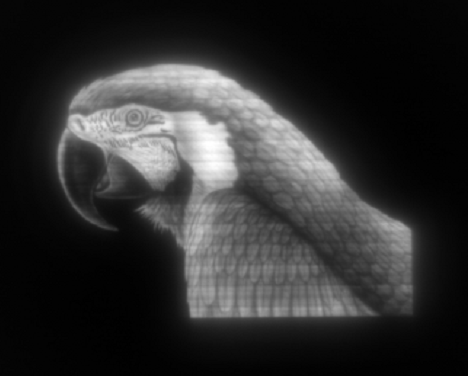
\includegraphics{fig/pdp_bird.png}
                \caption{Non-uniformity Corrected IR Image Drawn with PDP Firmware}
                \label{fig:pdp_bird}
            \end{figure}

            Figure~\ref{fig:pdp_grid} shows a grid being displayed on the same array. The lower right hand corner of the array has physical defects but the majority of the array operates correctly. Interdispersed in between the working pixels are a couple of dead pixels here and there. These look worse in a static grid map than in practice, as the brightness of neighboring pixels will hide individually defective pixels within an array. This is true as long as multiple pixels within a small region of an array are not defective as well. This is why Figure~\ref{fig:pdp_bird} has no obvious dead pixels.

            \begin{figure}[t]
                \centering
                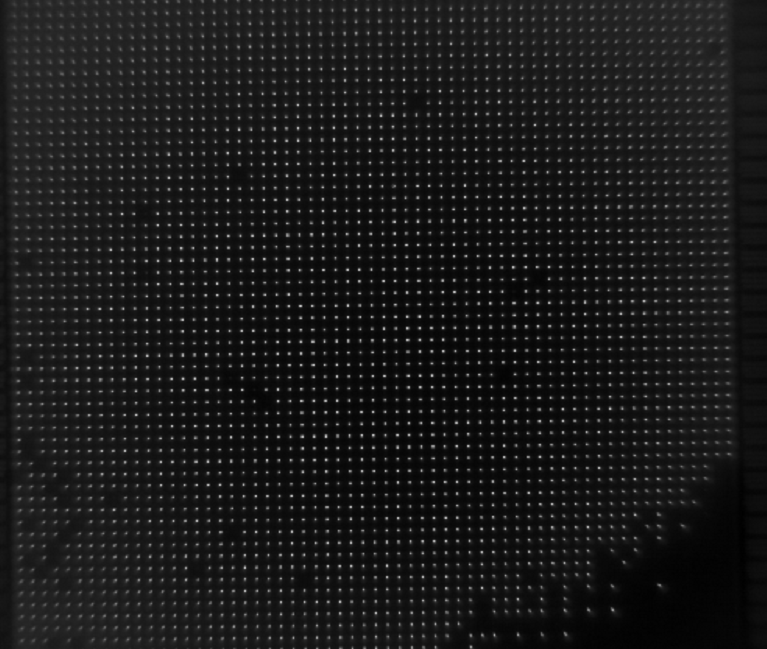
\includegraphics[width=0.6\textwidth]{fig/pdp_grid.png}
                \caption{Grid Drawn with PDP firmware}
                \label{fig:pdp_grid}
            \end{figure}


\section{Packetized Operation}
        This section shows various examples of PDP running at low-speed and high-speed operation to demonstrate the capabilities and versatility of a packetized display protocol.

    \subsection{Normal-speed}
        %60hz 240hz
        Figure~\ref{fig:low_speed_numbers} shows a series of counting numbers operating at low speeds. These were part of some of the initial demos used for testing packetized operation. This demo, in particular, ran at a number of different rates ranging from \mbox{60 hertz} to \mbox{240 hertz} operation.

        \begin{figure}
            \centering
            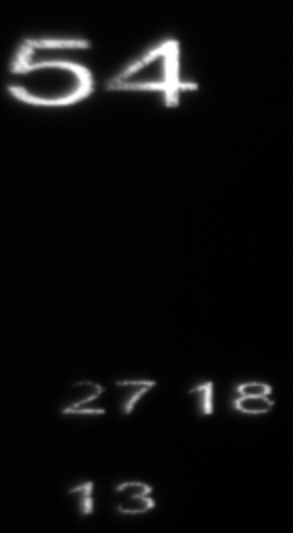
\includegraphics[width=0.15\textwidth]{fig/low_speed_numbers.png}
            \caption{60Hz to 240Hz Counting Demo Drawn with PDP Firmware}
            \label{fig:low_speed_numbers}
        \end{figure}

    \subsection{High-speed}
        There has been a number of different high-speed demos used to test PDP at rates above \mbox{250 Hz} operation on an NSLEDS array. Due to the limitations in IR Camera speed these were obtained by windowing the camera resolution down to allow for faster capture. Under full resolution, the IR camera used can only reach \mbox{565 Hertz}.

        Figure~\ref{fig:high_speed_object} shows a still image for a demo of an object that bounces at \mbox{1 kilohertz}. This object was drawn using multiple PDP draw region packets embedded into a larger HDMI frame. For every packet the {\it x start} and {\it y start} locations are modified. Drawing at this rate with normal full frame HDMI is impossible. At best, \mbox{240 Hertz} may be used with sacrifices in image brightness due to limited analog bandwidth.

        \begin{figure}
            \centering
            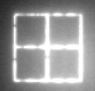
\includegraphics{fig/high_speed_object.png}
            \caption{1Khz Moving Object Displayed Drawn with PDP Firmware}
            \label{fig:high_speed_object}
        \end{figure}

        Figure~\ref{fig:high_speed_numbers} shows a series of images for a number counting demo running at {2 Kilohertz} operation. This demo ran both in a static predefined location as well as could be configured to move around the array. The object itself was drawn using individual PDP packets for each numerical digit. As with the previous example, drawing at this rate with normal full frame HDMI is impossible.

        \begin{figure}
            \centering
            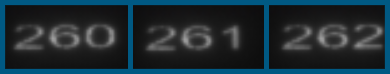
\includegraphics[width=0.6\textwidth]{fig/high_speed_numbers.png}
            \caption{2Khz Counting Demo Drawn with PDP Firmware}
            \label{fig:high_speed_numbers}
        \end{figure}

        Figure~\ref{fig:high_speed_rotating_object} shows a series of images for a non-uniformity corrected rotating three dimensional object running at {2 Kilohertz} operation. The object itself was drawn using individual PDP packets for each rotation. Notably, even with the limited resolution of the IR camera when operating at a high-speed, the object is clear and distinct during each rotation.

        \begin{figure}
            \centering
            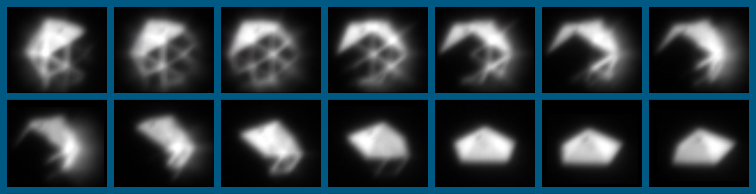
\includegraphics[width=0.6\textwidth]{fig/high_speed_rotating_object.png}
            \caption{2Khz Non-uniformity Corrected Rotating Object Drawn with PDP Firmware}
            \label{fig:high_speed_rotating_object}
        \end{figure}

%preliminary 2khz pdp demo:
%1900hz numbers counting to 1995
%camera 6200 at ~1950hz (need to update with camera config)
%nsleds 3 cyro with dio board
%note the last packet of every hdmi frame (running 100hz mode) is longer than every other packet due to %blanking, i believe this is the biggest contributor to the desync seen plus the camera rate isnt exactly matched
